%File: formatting-instruction.tex
\documentclass[letterpaper]{article}

% packages AIIDE
\usepackage{aaai}
\usepackage{times}
\usepackage{helvet}
\usepackage{courier}

% packages Sander
\usepackage{graphicx}
\usepackage{epstopdf}
\usepackage{amssymb}
\usepackage{amsmath}
\usepackage{url}
\usepackage{booktabs}												%% publication quality tables in latex
\usepackage{soul} 													%% for strikeout font effect
%\usepackage[utf8]{inputenc}
%\usepackage[algoruled,linesnumbered]{algorithm2e}
\usepackage{amsmath}
\usepackage[font=footnotesize]{caption}
\usepackage[font=scriptsize]{subcaption}
%\usepackage{subfig}
%\usepackage{subfigure}
%\usepackage{euler}
%\usepackage{breqn}
%\usepackage{algorithmic}

\usepackage{tikz}
\usepackage{amssymb}
\usetikzlibrary{calc}
\usetikzlibrary{positioning}
\usepackage{algorithm}
\usepackage[noend]{algpseudocode}
\usepackage{amsmath}
\usepackage{setspace}

\captionsetup[algorithm]{font=scriptsize}


% parameters AIIDE
\frenchspacing
\setlength{\pdfpagewidth}{8.5in}
\setlength{\pdfpageheight}{11in}

% parameters Sander
\widowpenalty=10000
\clubpenalty=10000
\widowpenalty=5000
\clubpenalty=5000
\interfootnotelinepenalty=10000

%\raggedbottom \topskip 1\topskip plus1pt 
%\flushbottom
%\raggedbottom
%\sloppy
%\sloppypar
%\frenchspacing

\hyphenation{na-me-ly know-led-ge}

\urlstyle{same}

%\SetAlgoCaptionSeparator{.}
%\renewcommand\AlCapFnt{\scriptsize\normalfont\scshape}

\setlength{\belowcaptionskip}{-3.4pt}

%\setlength{\floatsep}{-10pt}
%\setlength{\textfloatsep}{-5pt}

%\let\oldthebibliography=\thebibliography
%\let\endoldthebibliography=\endthebibliography
%\renewenvironment{thebibliography}[1]{%
  %\begin{oldthebibliography}{#1}%
    %\setlength{\parskip}{0ex}%
    %\setlength{\itemsep}{0ex}%
%}%
%{%
  %\end{oldthebibliography}%
%}



\pdfinfo{
/Title (Blinded for review)
/Author (Blinded for review)}
\setcounter{secnumdepth}{0}  
 \begin{document}
% The file aaai.sty is the style file for AAAI Press 
% proceedings, working notes, and technical reports.
%
\title{Towards Personalised Gaming via Facial Expression Recognition}
\author{\large{Paris Mavromoustakos Blom\textsuperscript{1}, Sander Bakkes\textsuperscript{1}, Chek Tien Tan\textsuperscript{2},}\\\large{\textbf{Shimon Whiteson\textsuperscript{1}, Diederik Roijers\textsuperscript{1}, Roberto Valenti\textsuperscript{1}, and Theo Gevers\textsuperscript{1}}}\\
\small{\textsuperscript{1}University of Amsterdam, Intelligent Systems Laboratory, Amsterdam, The Netherlands}\\
%paris.mavromoustakos-blom@student.uva.nl, \{s.c.j.bakkes, s.a.whiteson, d.m.roijers, r.valenti, th.gevers\}@uva.nl\\
\small{\textsuperscript{2}University of Technology, Games Studio, Sydney, Australia}\\
%chek@gamesstudio.org
}
\maketitle


\begin{abstract}
\begin{quote}
In this paper we propose two approaches for personalising the space in which a game is played (i.e., levels) dependent on classifications of the user's facial expression -- to the end of tailoring the affective game experience to the individual user. Our approaches are aimed at online game personalisation, i.e., the game experience is personalised \emph{during actual play} of the game. A key insight of this paper is that game personalisation techniques can leverage novel computer vision-based techniques to \emph{unobtrusively} infer player experiences automatically based on \emph{facial expression analysis}. Specifically, to the end of tailoring the affective game experience to the individual user, in this paper we (1) leverage the proven \textsc{InSight} facial expression recognition SDK as a model of the user's affective state \cite{InSight}, and (2) employ this model for guiding the online game personalisation process. User studies that validate the game personalisation approaches in the actual video game \textsc{Infinite Mario Bros.} reveal that it provides an effective basis for converging to an appropriate affective state for the individual human player.
\end{quote}
\end{abstract}
%We contribute an approach that acknowledges that for effective online game personalisation, one needs to rapidly converge to an appropriate policy for the individual user in online gameplay. To this end, we (1) utilise the proven \textsc{InSight} facial expression recognition SDK as a model of the user's affective state \cite{InSight}, and (2) employ this model for guiding the online game personalisation process. 
%Our approach specifically considers two design challenges, namely \emph{implicit user feedback} and \emph{high risk of user abandonment}. We contribute an approach that acknowledges that for effective online game personalisation, one needs to (1) offline learn a policy that is appropriate in expectation across users -- to be used for initialising the online game, (2) offline learn a mapping from gameplay observations to the player experience -- to be used for guiding the online game personalisation, and (3) rapidly converge to an appropriate policy for the individual user in online gameplay -- employing the learned feedback model and specific domain knowledge.
%%Our approach specifically considers two design challenges, namely \emph{implicit user feedback} and \emph{high risk of user abandonment}. We contribute an approach that acknowledges that for effective online game personalisation, one needs to (1) offline learn a policy that is appropriate in expectation across users -- to be used for initialising the online game, (2) offline learn a mapping from gameplay observations to the player experience -- to be used for guiding the online game personalisation, and (3) rapidly converge to an appropriate policy for the individual user in online gameplay -- employing the learned feedback model and specific domain knowledge.



\section{Introduction}

Ideally, artificial intelligence (AI) in games provides satisfactory and effective game experiences for players regardless of gender, age, capabilities, or experience \cite{CharlesMcNeill:2005}; it allows for the creation of personalised games, where the game experience is continuously tailored to fit the individual player. Indeed, we are now at a point where modern computer technology, simulation, and AI have opened up the possibility that more can be done with regard to \emph{on-demand} and \emph{just-in-time personalisation} \cite{riedl2010scalable}. However, achieving the ambition of creating personalised games requires the development of novel techniques for assessing online and unobtrusively which game adaptations are required for optimizing the individual player's experience.

The goal of this research is to online generate game spaces (i.e. levels) such that the spaces optimise player challenge for the individual player. A major challenge to this end, is that in online gameplay only implicit feedback on the appropriateness of the personalisation actions is available, i.e., the AI can only observe the player interacting with the game, while not being provided with labels on the player experience. Still, methods for tailoring the affective game experience to the individual user require an indication on how appropriate the provided experience is to the player. However, explicitly asking for player feedback during gameplay, is usually too intrusive, and would gravely affect the game experience. It is thus of the essence to use as much implicit feedback as possible, to obtain an as accurate as possible model of the player experience.

In order to achieve the aforementioned goal, we have developed two different implementations of an \emph{unobtrusive} system, namely a \emph{supervised} and an \emph{unsupervised} algorithm. The unsupervised version uses \textsc{InSight} output data to directly calculate the future difficulty of the game, while the supervised one uses a trained Random Forest classifier to predict a label of the user's current challenge level.

%Indeed, there is a strict need to derive feedback in a way that does not interfere with natural gameplay. 
%A key insight of this paper is that classifications of a users facial expression can be leveraged as an implicit model of a player's affective state, and this model can in turn be employed for tailoring the affective game experience to the individual user.

A key insight of this paper is that game personalisation techniques can leverage novel computer vision-based techniques to \emph{unobtrusively} infer player experiences automatically based on \emph{facial expression analysis}. Specifically, to the end of tailoring the affective game experience to the individual user, in this paper we (1) leverage the established \textsc{InSight} facial expression recognition SDK as a model of the user's affective state \cite{InSight}, and (2) employ this model for guiding the online game personalisation process.
%%Motivated by this need, we build on prior work [27] that proposes a novel computer vision-based technique to infer player experiences automatically based on \emph{facial expression analysis}. 
%Motivated by the need to capture data in a way that does not affect natural gameplay, we build on prior work [27] that proposes a novel computer vision-based technique to infer player experiences automatically based on \emph{facial expression analysis}. Facial expression analysis [12] is the use of automatically recognized facial expressions to infer affective states. It is a video based approach which is non-obtrusive compared to current physiological approaches. This allows for a more authentic play experience and enables data collection in non laboratory settings.
%in online gameplay we rapidly converge to an appropriate policy for the individual user. To do this well, we employ the learned feedback model and specific domain knowledge to effectively guide state-space exploration.

As such, we consider challenge to be a cognitive state that might incorporate affective patterns that could be expressed through the face. We focus purely on attaining an appropriate challenge level through the online learning from affective signals; a relatively challenging task. This operates by adjusting procedural parameters that control the intended challenge level -per content type- within the game. This provides expressiveness to tailor the intended challenge level to specific users (by adapting specific content in a distinct manner). Specifically, we will control the \emph{intended} challenge level based on measured affective states; we do not make assumptions on the relationship of affect and challenge.



%User studies that validate the personalisation approach in the actual video game \textsc{Infinite Mario Bros.} reveal that (1) the online personalisation method operates as expected -- it decreases specific challenge levels in the face of user anger, and increases specific challenge levels in the face of user neutrality or happiness -- and appears stable in the face of classification noise, and (2) a significant majority of human participants prefers the personalised gaming system over the static system. We therefore conclude that our game personalisation approach -- built upon facial expression analysis -- provides an effective basis for converging to an appropriate affective state for the individual human player.
%in online gameplay our approach can balance the game's challenge level such that it is appropriate to the individual user, and (2) in pairwise tests, human participants prefer our personalised gaming system over a static gaming system.
%User studies that validate the game personalisation approach in the actual video game \textsc{Infinite Mario Bros.} reveal that it provides an effective means for converging to an appropriate affective state for the individual human player.

%This entails two challenges, namely (1) in online gameplay only implicit feedback on the appropriateness of the personalisation actions is available (i.e., the AI can only observe the player interacting with the game, while not being provided with labels on the player experience), and (2) there is a high risk of user abandonment when inappropriate game personalisation actions are performed.

%Our contribution is an approach built on three features that address these challenges. Addressing the first challenge, a feedback model needs to be learned which maps gameplay observations to an estimate of the player experience. The feedback model is learned offline and is subsequently employed for decision-making in online gameplay. Addressing the second challenge, a policy needs to be learned that is appropriate in expectation across users. This policy is learned offline and is subsequently employed to safely initialise online gameplay. Also addressing the second challenge, in online gameplay we rapidly converge to an appropriate policy for the individual user. To do this well, we employ the learned feedback model and specific domain knowledge to effectively guide state-space exploration.

%Experiments that validate our approach in the actual video game \textsc{Infinite Mario Bros.} reveal that (a) in online gameplay our approach can balance the game's challenge level such that it is appropriate to the individual user, and (b) in pairwise tests, human participants consistently prefer our personalised gaming system over a static gaming system.



\section{Game Personalisation}\label{sec:gamepersonalisation}

Game personalisation is motivated by a significantly increased involvement and extensive cognitive elaboration when subjects are exposed to content of personal relevance \cite{petty1979issue}; they will exhibit stronger emotional reactions \cite{darley1992effect}. Particularly, a positive effect on player satisfaction is indicated, i.e., game personalisation raises player loyalty and enjoyment, which in turn can steer the gaming experience towards a (commercial) success \cite{teng2010customization}. Indeed, the perspective of AI researchers to increase the engagement and enjoyment of the player is one that is consistent with the perspective of game designers \cite{riedl2010scalable}, i.e., personalisation methods are regarded as instrumental for achieving industry ambitions \cite{Molyneux:2006}. Tailoring the game experience to the individual player particularly benefits from the use of player models, and requires components that use these models to adapt part of the game \cite{bakkes2012personalised-journal}.

Our research follows the emerging trend of employing AI methods for adapting the game environment itself (as opposed to, more typically, adapting the behaviour of the game characters) \cite{Bakkes:ChallengeBalancing}. In our investigation, we choose to focus on \emph{personalising the game space} to the individual player with respect to experienced challenge. Related work with regard to this scope is discussed next.
%\footnote{Abstractly speaking, we consider the game space to be the representation of the game mechanics through which the user interacts with the game. Typically, in a video game setting, the game space will be the levels in which the game takes place. Game space personalisation, in this context, generally concerns the online learning of the next set of level design parameters.}

%This section reviews literature related to the general domain of player experience analysis and provides some background on the facial expressions analysis techniques applied in ways similar to our goals.

\subsection{Player Experience Analysis}

We build on the novel perspective that computer vision techniques can automatically infer gameplay experience metrics \cite{Tan2012,tan2012feasibility}, a field broadly categorized into qualitative and quantitative methods.
%The motivations for this research is derived from the state of current research and practice in the area of player experience analysis, which is

Qualitative methods involve the collection and analysis of subjective data for games; this often includes direct observations, interviews and think-aloud protocols. These methods are most common amongst game practitioners and usually require formal playtest sessions in artificial play environments \cite{tan2012feasibility}. Although these methods have been shown to usually reflect accurate states, they have several shortcomings. Firstly, they might inhibit true play experiences, as players might not be totally at ease when someone is watching or questioning them. Players might not be able to properly self-articulate their play experiences concurrently during gameplay and might not remember important details when post interviews are performed. Secondly, the sessions also often require a lot of time and resources to conduct and analyze. Hence there is a need for more efficient, accurate and versatile (ability to conduct in non-laboratory settings) ways to perform player experience analysis.

These reasons have driven much research towards quantitative methods that work on objective data. Quantitative methods have the potential to represent true player experiences in the game and are able to continuously capture a more diverse body of information. Common approaches include telemetry and psychophysiology.

Telemetry primarily deals with the logging of player in-game interactions to build player models, and several studies have been performed \cite{Zammitto2010,Medler2011,Moura2011,Gagne2011}. The advantage of Telemetry over qualitative methods is that it is non-disruptive and that it can continuously capture objective gameplay statistics in non-laboratory settings. However, the data is limited to the in-game actions available to the player and events in the game world. Hence these ``virtual observations" do not capture full experiences and might not even represent the true experiences of the player in real life. For example, a player might take a long time to clear a level, but he might be having a high level of arousal in real life, having fun exploring the level, or simply be stimulated by the aesthetics.

Psychophysiology is the other main branch of quantitative player experience research, which consists of methods to infer psychological states from physiological measurements, that commonly include electrodermal activity (EDA), electromyography (EMG), electrocardiogram (ECG), electroencephalography (EEG), body temperature and pupil dilations. Current work \cite{Mandryk2006,Nacke2008,yannakakis2009real,Nacke2010,Zammitto2010,Drachen2010} mostly involve inferring emotional valence and arousal by employing a combination of the measurements. Amongst them, EDA and EMG seems to be most popular as they correspond accurately to emotional dimensions of arousal and valence respectively \cite{Russell1980}. Similar to telemetry, physiological measurements are able to capture player experiences continuously in real-time. In addition, physiological data represent the real life experiences of the player. Unfortunately, most current approaches deal with expensive specialised equipment that are obtrusive, which are usually only viable in controlled laboratory settings. As such, we propose to investigate using a video-based approach to capture data in way that is more efficient, versatile, and does not affect natural gameplay.
%These reasons have led to the position we have taken to propose the investigation of using a video-based approach to capture data in way that is more efficient, versatile, and does not affect natural gameplay.
%The approach we will start with is the established technique in computer vision - facial expressions analysis.

\subsection{Facial Expression Recognition}

The first step in any facial expressions analysis system is to recognize facial expressions; being a fairly mature domain in computer vision with techniques that boast a high level of accuracy and robustness \cite{Bartlett1999,Michel2003,buenaposada2007,McDuff2011}. For example, Buenaposada et al. \citeyear{buenaposada2007} have reported an 89\% recognition accuracy in video sequences in unconstrained environments with strong changes in illumination and face locations.

In terms of using it for analysis of user experiences, there has been a limited number of works performed in non-game applications \cite{Branco2006,Zaman2006}. Branco \citeyear{Branco2006} showed some encouraging results evaluating positive and negative expressions of users of an online shopping website. Zaman and Shrimpton-Smith \citeyear{Zaman2006} evaluated an automated facial expressions analysis system to infer emotions that users had whilst performing common computer usage tasks. They generally reported a high level of correlation between the system's findings and human expert analyses. In other domains, general emotion detection based on facial expression recognition \cite{Ghijsen2004,Baltrusaitis2011} have also shown promising results.  

In our research, we take the distinct focus of balancing the game's challenge level by adapting the \emph{content} that is placed within the game environment dependent on facial expression analysis. Particularly, we focus on procedural content generation (cf. Togelius et al. \citeyear{togelius2011search}; Yannakakis \citeyear{Yannakakis2011a}) for tailoring the player experience. Our distinct focus in this matter, is to assess \emph{online} and \emph{unobtrusively} which game adaptations are required for optimizing the individual player's experience while the game is being played, so as to have assessments on the experienced player challenge impact the procedural process (\emph{cf}. Bakkes et al. \citeyear{Bakkes:ChallengeBalancing}).




%Player modelling is of increasing importance in modern video games \cite{Furnkranz:2007}; it is almost a necessity when the purpose of AI is `entertaining the human player' rather than `defeating the human player' \cite{Herik:OM}. A challenge for player modelling in video games is that models of the player have to be established (1) in game environments that generally are relatively complex, (2) with typically little time for observation, and (3) often with only partial observability of the environment \cite{lankveldpersonalityprofiling,bakkes2012player}. A recent development with regard to player modelling is to automatically establish psychologically or sociologically verified player profiles \cite{bakkes2012player}. Such models provide motives or explanations for observed behaviour. A solid profile can be used to, for instance, predict a player's affective state during play of the game. 
%In our research, we take the distinct approach of utilising player models for the purpose of optimising the player experience (\emph{cf.} the work of Yannakakis \emph{et al.} \citeyear{yannakakis2009real}).

%\subsection{Challenge balancing}\label{sec:components-difficultyscaling}
%
%Challenge balancing concerns automatically adapting the challenge that a game poses to the skills of a player \cite{Olesen:2008,Spronck:DifficultyScaling}. It aims at achieving a `balanced game', i.e., a game wherein the player is neither challenged too little, nor challenged too much. In most games, the only implemented means of challenge balancing is provided by a \emph{difficulty setting}, i.e., a discrete parameter that determines how challenging the game will be. However, as the challenge provided by a game is typically \emph{multi-faceted}, it is hard for the player to estimate reliably the challenge level that is appropriate for her. Furthermore, generally only a limited set of discrete difficulty settings is available (e.g., easy, normal, hard). This entails that the available settings are not fine-tuned to be appropriate for each player. As such, researchers have developed advanced techniques for balancing the challenge level of games. Hunicke and Chapman \shortcite{Hunicke:2004} explored challenge balancing by controlling the strength of opponent characters (i.e., controlling the opponent character's health, accuracy, and employed weapons). Spronck \emph{et al.} \shortcite{Spronck:DifficultyScaling} investigated methods for automatically adjusting weights assigned to possible game scripts. Indeed, knowledge on the specific effect of game adaptations can be employed for maintaining a challenge level \cite{Bakkes:RapidReliable}, and may be incorporated to steer the procedural generation of game content \cite{togelius2011search}.
%
%In our research, we take the distinct focus of balancing the game's challenge level by adapting the \emph{content} that is placed within the game environment.

%\subsection{Space adaptation}\label{sec:components-space}
%
%Game space adaptation concerns allowing the space in which the game is played to adapt, ideally in response to the user experience \cite{dormansbakkes:2011}. Game space adaptation is an active area of research \cite{togelius2011search,togelius2010towards,pedersen12modeling,dormansbakkes:2011,smith2009rhythmbased}, which falls within the scope of experience-driven procedural content generation \cite{yannakakis2011experience}. Research is increasingly focussing on how procedural techniques may be employed specifically for enhancing the player experience. For example, the feasibility of procedurally generating a personalised race track has already been demonstrated by Togelius et al. \shortcite{togelius2006making,togelius2007towards}. We briefly highlight three distinct investigations that have been performed in the context \emph{personalised procedural content generation}. Adrian \emph{et al.} \shortcite{adrian2013approach} and Traichioiu \emph{et al.} \shortcite{Traichioiu2014} investigated the procedural generation of levels with respect to a difficulty curve. Dormans and Bakkes \shortcite{bakkesinvolving,dormansbakkes:2011} investigated the procedural generation of entire levels for action-adventure games, which distinguishes between missions and spaces as two separate structures that need to be generated in two individual steps. Lopes \emph{et al.} \shortcite{LTB12a} developed a framework aimed at creating personalised content for complex and immersive game worlds; by modelling which content provided the context for a given personal gameplay experience. Bakkes et al. \shortcite{Bakkes:ChallengeBalancing} investigated personalising the space in which a game is played (i.e., levels) -- to the end of tailoring the experienced challenge to the individual player during actual play of the game.
%
%In our research, we also focus on procedural content generation for tailoring the player experience. Our distinct focus in this matter, is to assess \emph{online} and \emph{unobtrusively} which game adaptations are required for optimizing the individual player's experience while the game is being played, so as to have assessments on the experienced player challenge impact the procedural process (\emph{cf}. Bakkes et al. \citeyear{Bakkes:ChallengeBalancing}).


%\subsection{Player modelling}\label{sec:components-playermodelling}
%
%Player modelling is of increasing importance in modern video games \cite{Furnkranz:2007}; it is almost a necessity when the purpose of AI is `entertaining the human player' rather than `defeating the human player' \cite{Herik:OM}. A challenge for player modelling in video games is that models of the player have to be established (1) in game environments that generally are relatively complex, (2) with typically little time for observation, and (3) often with only partial observability of the environment \cite{lankveldpersonalityprofiling,bakkes2012player}. A recent development with regard to player modelling is to automatically establish psychologically or sociologically verified player profiles \cite{bakkes2012player}. Such models provide motives or explanations for observed behaviour. A solid profile can be used to, for instance, predict a player's affective state during play of the game. 
%
%In our research, we take the distinct approach of utilising player models for the purpose of optimising the player experience (\emph{cf.} the work of Yannakakis \emph{et al.} \citeyear{yannakakis2009real}).



\section{Domain description}\label{domain}

We consider a typical video game: \textsc{Infinite Mario Bros.} \cite{infiniteMario}; an open-source clone of the classic video game \textsc{Super Mario Bros.} It can be regarded an archetypal platform game; despite its relatively straightforward appearance it provides a diverse and challenging gameplay experience. We build upon a version of \textsc{Infinite Mario Bros.} that has been extended to procedurally generate entire Mario levels. These extensions have been made by Shaker \emph{et al.} \shortcite{shaker2011game,shaker2012digging,shaker2013crowdsourcing}, Pedersen \emph{et al.} \shortcite{pedersen2009modeling,pedersen12modeling}, and Togelius \emph{et al.} \shortcite{togelius20102009}.

We have made two further enhancements to the 2011 Mario AI Championship game engine of \textsc{Infinite Mario Bros.} First, it now is able to procedurally generate \emph{segments} of Mario levels while the game is in progress (Figure~\ref{fig:mario}). Second, we can now inject short \emph{chunks} of specific game content: (1) a straight chunk, containing enemies and jumpable blocks, (2) a hill chunk, also containing enemies, (3) a chunk with tubes, containing enemy plants, (4) a jump, and (5) a chunk with cannons. Each chunk can have six distinct implementations, stemming from a per-chunk parameter value $\in [0,5]$. The challenge level of the chunk monotonically increases with the parameter value. In online gameplay, the only action that the personalisation algorithm can take is to output a vector of five integers (chunk parameters) $\in [0,5]$ to the procedural process which in turn generates the next level segment. While the action space is relatively modest in size, its resulting expressiveness ranges from overly easy to exasperatedly hard level segments.

%We have made two further enhancements to the 2011 Mario AI Championship game engine of \textsc{Infinite Mario Bros.} First, we enhanced the engine such that it is able to procedurally generate \emph{segments} of Mario levels while the game is in progress (Figure~\ref{fig:mario}). One game segment has a width of 112 game objects, and generally takes a player approximately 20 to 30 seconds to complete. This enhancement enables feedback on the observed player experience to rapidly impact the procedural process that generates the upcoming level segments. The upcoming level segments are generated seamlessly, such that no screen tears occur when the user is transitioning from one segment to the next (i.e., before the next segment can be observed a short `gap' block is injected in the game space).

\begin{figure}[t]
  \begin{center}
  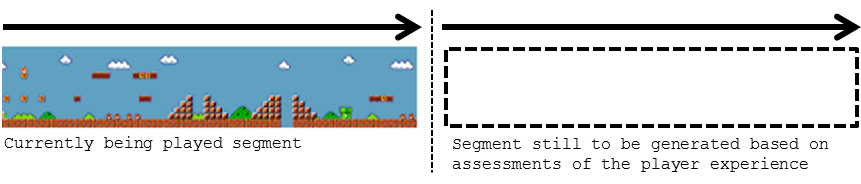
\includegraphics[width=1.00\columnwidth]{images/mario-new-new-new-new.png}
  \caption{Our enhanced version of \textsc{Infinite Mario Bros.} During gameplay it generates short \emph{new level segments} of specific content \emph{on-the-fly}, on the basis of classifications of the facial expression.}
  \label{fig:mario}
  \end{center}
\end{figure}

%Our second enhancement to the game engine, is that within every segment we can now inject short \emph{chunks} of specific game content. We enabled the game engine to generate five different types of chunks, (1) a straight chunk, containing enemies and jumpable blocks, (2) a hill chunk, also containing enemies, (3) a chunk with tubes, containing enemy plants, (4) a jump, and (5) a chunk with cannons. Each chunk can have six distinct implementations, stemming from a per-chunk parameter value $\in [0,5]$. The challenge level of the chunk monotonically increases with the parameter value (e.g., a hill parameter value of 0 entails a chunk with no hills and no enemies, while a value of 5 entails five procedurally-generated hills with five relatively difficult enemies). Our enhanced engine has the desired property that the generated chunks are largely independent of each other, i.e., only in rare cases will one chunk be able to affect player behaviour in the surrounding chunks (e.g., in case a cannon bullet follows the player to the next chunk). To benefit playability and level aesthetics, the order in which the chunks are encountered is randomized for each new segment. The five chunks (each 16 game objects in length) - concatenated in random order - are preceded and succeeded by a flat, neutral chunk (also 16 game objects in length), to allow the player to prepare for the next game segment.

%In online gameplay, the AI that personalises the game space is input with a vector of 60 real-numbered features values, the standard logging capability of the game's data recorder (45 features) appended by hand-coded features (15 features). The features concern observed player behaviour (e.g., how much time did it take the player to complete the segment) (\emph{cf.} \citeauthor{shaker2011game} \citeyear{shaker2011game}). The only action that the AI can take is to output a vector of five integers (chunk parameters) $\in [0,5]$ to the procedural process which in turn generates the next level segment. While the action space is relatively modest in size, its resulting expressiveness ranges from overly easy to exasperatedly hard level segments.




\section{Unsupervised Approach}\label{sec:approach}

The goal of this approach is to online generate game spaces (i.e. levels) such that the spaces optimise player challenge for the individual player. To this end, a key insight is that game personalisation techniques can leverage novel computer vision-based techniques to \emph{unobtrusively} infer player experiences automatically based on \emph{facial expression analysis}. We perform emotion tracking, with the established \textsc{InSight} facial expression recognition SDK \cite{InSight}, and gradient ascent optimisation of the individual game experience.
%. The classifications on the player's facial expression serves as input in a gradient ascent optimization system that on-line determines the challenge level of specific content (chunks) in the game (e.g., a chunk consisting of cannons, a chunk consisting of a jump, etc.).
%The main challenge in this respect is making accurate assessments of the player's expressions while (s)he is playing the game, and mapping these assessments into challenge levels that are appropriate to the observed player.
%The present research aims towards optimizing player experience through intelligent game level generation.

\subsection{Emotion tracking}

In our approach, player emotions are tracked with the \textsc{InSight} facial expression recognition SDK \cite{InSight} through the duration of a game session, yet are taken into account real-time and are chunk specific. As such we are not measuring, e.g., general happiness, but instead can map (parameters that generated) specific game content to specific affective states. We hereby assume that the classification probability of an affective stance indicates how strongly it is expressed by the player.
%That is, player expressions measured in chunk $c$ (e.g., a chunk with cannons as content), will in our approach only affect the challenge level of that particular chunk. As a result, online personalisation is achieved at the \emph{content level} of the game. Indeed, this characteristic allows the online personalisation to specifically tailor the challenge level of a certain content type, to the measured affective state of the human player when interacting with this content.
%, with a wide variety of challenge levels can be reached within a single segment, adapting to the users' preferences regarding game chunks.

\textsc{InSight} classifies facial expressions at approximately 15 frames per second. For each frame, it outputs a probability distribution over seven distinct emotions, namely (1) neutrality, (2) happiness, (3) disgust, (4) anger, (5) fear, (6) sadness, and (7) surprise. Depending on the progress of the player through the Mario game, a game chunk is typically interacted with for 2 to 10 seconds, resulting in a total of 30 to 150 classifications for each game chunk separately. The resulting probability distributions are averaged at the end of each chunk, into an estimate of a players's emotional stance; it is an estimate that is relatively insensitive to classification noise of the facial expression system (which may occur in individual frames). \textsc{InSight} has an average accuracy of 93.2\% over all classified emotions \cite{InSight}.

There are two events at which assessments on the player's affective state are used to adapt the game; namely (1) when the next level segment needs to be generated, and (2) when the game resets due to player death. To this end, we take into consideration not only player assessments made during actual play of the game, but also in between in-game deaths of the human player -- as we observed that during this observational period many game players express high emotional activity. Furthermore, we particularly consider that -- following our experience with the target domain -- most game players tend to maintain a relatively neutral facial expression during gameplay, with most emotional `bursts' occurring when human players experience an in-game death. Figure~\ref{fig:emotions10seg} supports this intuition; it illustrates that `neutral' is the dominant affective stance, as measured for one player over the course of a game play session of approximately ten minutes, with bursts of anger, happiness, and sadness being measured as well.
%Furthermore, player emotions are taken into consideration during in-game death, which leads to a short game pause of a few seconds. It has been observed that during that period, users show high emotional activity, which we consider essential for the calibration of game difficulty.	It is a fact that a vast majority of the users tend to keep a neutral expression during game activity while most emotional "bursts" occur while players experience in-game death. As shown in Figure \ref{fig:emotions10seg}, neutral is the dominating emotion recorded in almost the entire course of 10 game segments, while spikes and bursts of anger, happiness and sadness are also present.

\begin{figure}[t]
	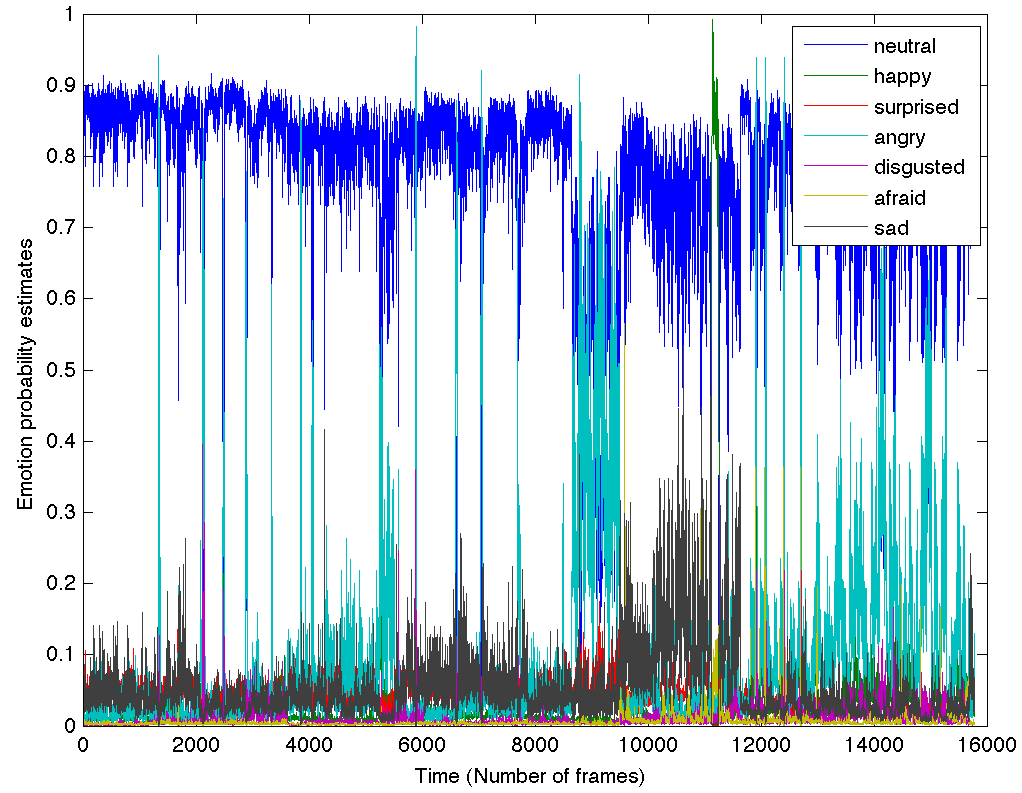
\includegraphics[width=1.00\columnwidth]{images/paris/allEmotions.png}
	\caption{Classifications of the facial expressions of one human participant, over the course of a ten-minute game playing session. We observe that the dominant affective stance is `neutral'.}
	\label{fig:emotions10seg}
\end{figure}

During actual play of the first segment of each game session, we calculate the variance in classification of each emotional stance $e$, from which we derive a factor $\alpha = 1 - var(e_1)$. This factor $\alpha$ is employed as a baseline for the gradient ascent algorithm; it aims at assessing the ``emotional expressiveness'' of each individual player. In our approach, the lower the variance in affective states (i.e., an observed player is not very expressive), the larger the gameplay adaptations to specific chunks when emotional bursts actually do occur (in either direction of intended challenge), considering that $var(e_1)$ is higher when a user shows high emotionality levels. Factor $\alpha$ is then multiplied to thresholds defined in the gradient ascent optimiser.
%the less emotional a player is considered to be, the higher the impact of a measured burst of emotions will have on adaptations to the game's challenge level
% and thus adapting these to each individual user.
%the calculations of the level generator.

\subsection{Gradient Ascent Optimisation}

To map classifications of the human player's facial expressions to appropriate in-game challenge levels, we employ a Gradient Ascent Optimisation (GAO) technique. It is employed for optimising the challenge levels for each content type in the game (i.e., for each chunk) such that human interactions with the content yield affective stances that have positive valence (i.e., happiness), while minimising affective stances that have negative valence (i.e., neutrality and anger).

Our implementation of GAO is relatively straightforward (Algorithm~\ref{euclid}). After a game segment has been completed by the human player, the probability-distribution vector of the measured emotional stances are retrieved for each individual chunk. The emotions taken into consideration for the present experiments are (1) neutrality, (2) happiness, and (3) anger; our preliminary trials with the Mario game suggested that these emotions were most likely to be expressed by human players (\emph{cf}. Figure~\ref{fig:emotions10seg}).

\begin{algorithm}[t]
\tiny
\caption{Facial Expression-based Gradient Ascent Optimisation}
\label{euclid}
\begin{algorithmic}[1]
\Procedure{GAOptimize}{$e_t,e_{t-1}$}\Comment{Emotion vectors of current and previous segment}

   \State $\alpha\gets 5*(1-Var(e_1))$\Comment{Calculate $\alpha$, scale to action space}

      \For{$each : chunk$}
      \If{playerDies(t)}
\State $\phi = round(5*\alpha * e_t[Anger])$
\State $chunk.decreaseChallengeLevel(\phi)$
\ElsIf{segmentFinished(t)}
\If{$e_t[Neutral]<= 0.8*\alpha$}
	\State $chunk.decreaseChallengeLevel(1)$
\Else
      \State $\epsilon\gets argmax_e|e_t-e_{t-1}|$ 
      \State $nextAction\gets round(\epsilon*\alpha)$
      \If{$e\in\{angry,neutral\}$}
      \State{$nextAction \gets -nextAction$}
      \EndIf
       \State{$nextChallengeLevel\gets previousChallengeLevel + nextAction$}
      \State \textbf{return} $newChallengeLevel$
      \EndIf

      \EndIf
   \EndFor
\EndProcedure
\end{algorithmic}
\end{algorithm}

At each iteration of GAO, when a game segment is finished, the emotion vectors -- of each individual chunk -- of the recently played (finished) segment $(S_t)$, plus the previously completed segment $S_{t-1}$, are fed into the algorithm. For each emotion that is taken into consideration (neutrality, happiness and anger), the difference between its current $(e_t)$ and previous iteration $(e_{t-1})$ value is obtained. Next, the maximum of the three differences is determined, namely $argmax(e_t-e_{t-1})$. Since the three emotions are equally weighted, the maximum value calculated could be considered as the ``most significant'' change in emotional status of the user between two game segments. This value can be considered the desired challenge level of the next segment, $S_{t+1}$. Since emotions are probabilistic estimates, their difference between two segments follows $D_{e}\in[-1...1]$. In order to determine the next segment's challenge level per chunk, $D_{e}$ has to be scaled up to action space of the employed procedural level generator of the Mario game, namely $[0...5]$. Thus, action $a_{t} = round(5D_{e}), a_{t}\in[-5...5]$ is calculated and defines the change in challenge level that will be presented in the next segment, where negative values define a drop in challenge and positive values define a respective increase. To summarize, the challenge level of a chunk in the next segment will be: $d_{S_{t+1}} = d_{S_{t}}+a{t}$. This calculation will be individually applied to all chunks within a game segment. In practice, the algorithm will increase the game challenge level if the probability estimate of an emotion is higher in timestep $t$ compared to $t-1$. However, we condition on which emotion is the one defining $a_t$, for the reason that an increase in ``negative'' emotions (neutrality and anger) should generate a decrease in game difficulty. That is why in these cases, we consider $a_t$ to be $-a_t$.
%%the segment's emotion vectors are fed into the algorithm. It is important to note that GAO keeps track of emotions deriving from both the recently finished segment $(S_t)$, and the previously completed one $S_{t-1}$, for each chunk individually. 
%An algorithmic representation of the iterative GAO procedure is shown in Algorithm ~\ref{euclid}.

In order to tailor GAO to the specific target domain, heuristic values are introduced in special occasions; all heuristic values follow from experimentation. Generally, as mentioned, users tend to show highly neutral expressions during gameplay, especially in gameplay settings of low challenge level. In order to prevent ``stalling'' the game at a certain challenge level due to lack of expressed emotionality, we introduce a heuristic threshold $\tau = 0.8\alpha$. The threshold is derived from our observations on player behaviour in the Mario game (Figure \ref{fig:emotions10seg}). If, by the end of a game segment, the level of neutrality of a player during a chunk was higher than the theshold $\tau$, the level generator will force an increase in challenge by a unit measure (+1) in the next segment's respective chunk. This heuristic corresponds to the insight that the possibility of failure (and the positive affect that is provided by overcoming an obstacle) is an important factor to an appropriate game experience \cite{juul2013art}.

On the other hand, lasting, excessively high challenge levels may impose an unpleasant experience on game players. In order to avoid player abandonment resulting from an inappropriately high challenge level, a second heuristic is applied onto emotions observed during in-game death. A threshold $\phi = 5\alpha\times\epsilon_{anger}$ is introduced regarding the anger measurement during death. The chunk in which death happened will instantly drop by $round(\phi)$ units of challenge level in an attempt to reduce player anger and boost player progress in the game. Note that $\epsilon_{anger} \in \{0...1\}$ is multiplied by $5$ in order to directly map emotion probability scale into game challenge scale.




\section{Experiments}\label{sec:experiments}

Here we discuss the experiments that validate our approach in the actual video game \textsc{Infinite Mario Bros.}

\subsection{Online personalisation -- Pilot study}\label{exp1}

In the pilot study, we analyse the personalisation system's performance by observing one human participant interact with the system under controlled experimental conditions. The participant is placed in a room with stable lighting conditions, and is instructed to interact with the personalised Mario game as she would at home, while attempting to refrain from blocking the face (e.g., by moving a hand through the hair, drinking coffee, etc.). The participant will interact with the game for ten minutes, starting at an initial challenge level of `easy' (all parameter values being `1'). Our hypothesis is that when facial expressions can be classified accurately, our online personalisation method will converge to a challenge level that yields an appropriate affective state for the user.

Figure~\ref{fig:emotions} illustrates the obtained results. For all chunks (Figure~\ref{fig:sectionStraightEmotions} -- \ref{fig:sectionCannonsEmotions}), we observe the general trend where the algorithm decreases the per chunk challenge levels (Figure~\ref{fig:sectionCannonsEmotions}) in the face of user anger, and increases the challenge levels in the face of user neutrality or happiness. Thereby, the online personalisation method operates as expected. For instance, Figure~\ref{fig:sectionDifficultiesEmotions} reveals that the challenge level for the cannons chunk (Figure~\ref{fig:sectionCannonsEmotions}) is initially increased because of high neutral levels. However, later in the game, high anger levels cause a drop in the challenge level. When lastly the angry emotion disappears, the challenge level becomes stable as well. Furthermore, in Figure~\ref{fig:sectionStraightEmotions} we observe that the online personalisation method appears stable in the face of classification noise. That is, after approximately 1000 classified frames, the human player suddenly expresses a `mix' of emotions; denoting, in practise, that the player is talking or moving too much. As expected, the associated challenge level (see Figure~\ref{fig:sectionDifficultiesEmotions}) remains stable in the face of this noise from the facial expression classifier.
%In addition, as expected, we observe that the challenge level for cannons (Figure~\ref{fig:sectionDifficultiesEmotions}) - after an initial increase due to relatively high neutral expressions - is decreased corresponding to measured anger of the player (Figure~\ref{fig:sectionCannonsEmotions}).
%As observed in Figure \ref{fig:difficulties10seg}, starting from an "easy" difficulty setting for each game chunk, GAO adapts and converges according to the player's preferences in the course of 10 segments.
%Indeed, it is important to consider that situations in which the facial expression cannot be classified reliably, is one that cannot be avoided in actual gameplay conditions.
%Also, fig2 (b) in the end we see a "mix" of many emotions, this denotes a player talking or moving too much and shows how the facial expression recognition system is really sensitive and can produce false classifications.
%Also, fig2 (d) tubes difficulty stays at 1 meanwhile the user seems neutral. that happens because his neutral levels are below the threshold α*0.8, so no difficulty adaptation is observed.

\begin{figure*}[t]
        \centering
        \begin{subfigure}[t]{0.32\textwidth}
								\centering
                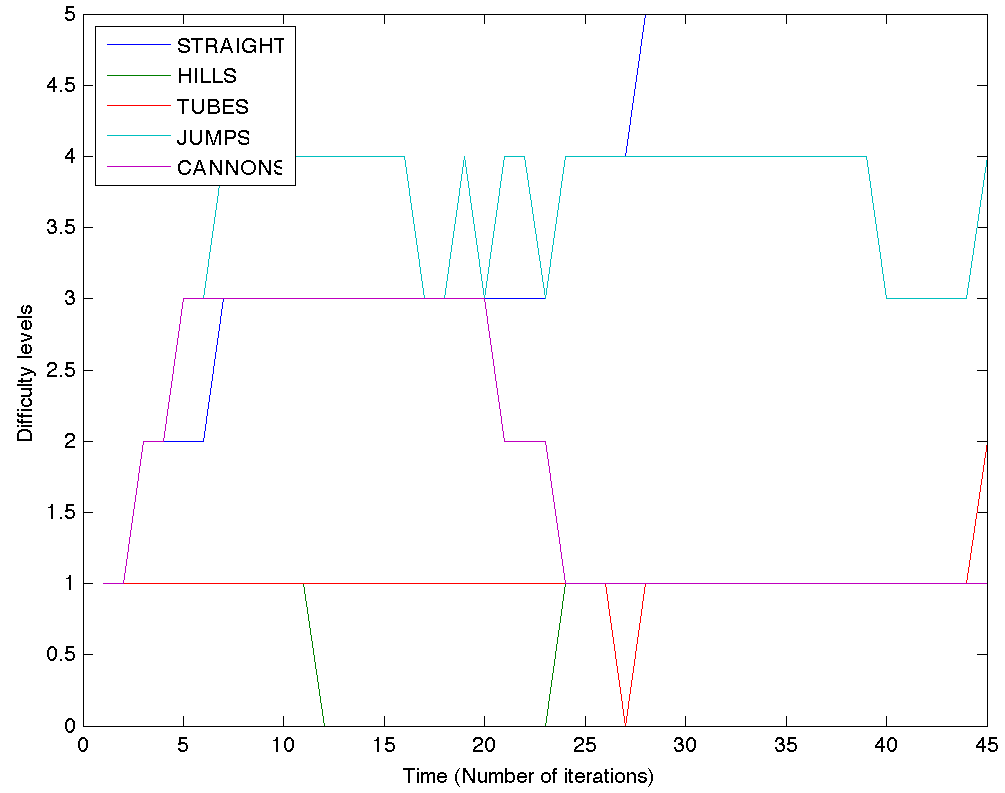
\includegraphics[height=4.7cm,keepaspectratio]{images/paris/difficulties.png}
                \caption{Challenge parameter values}
								\label{fig:sectionDifficultiesEmotions}
        \end{subfigure}%
				\quad
        %\\ %add desired spacing between images, e. g. ~, \quad, \qquad etc.
           %(or a blank line to force the subfigure onto a new line)
        \begin{subfigure}[t]{0.32\textwidth}
								\centering
                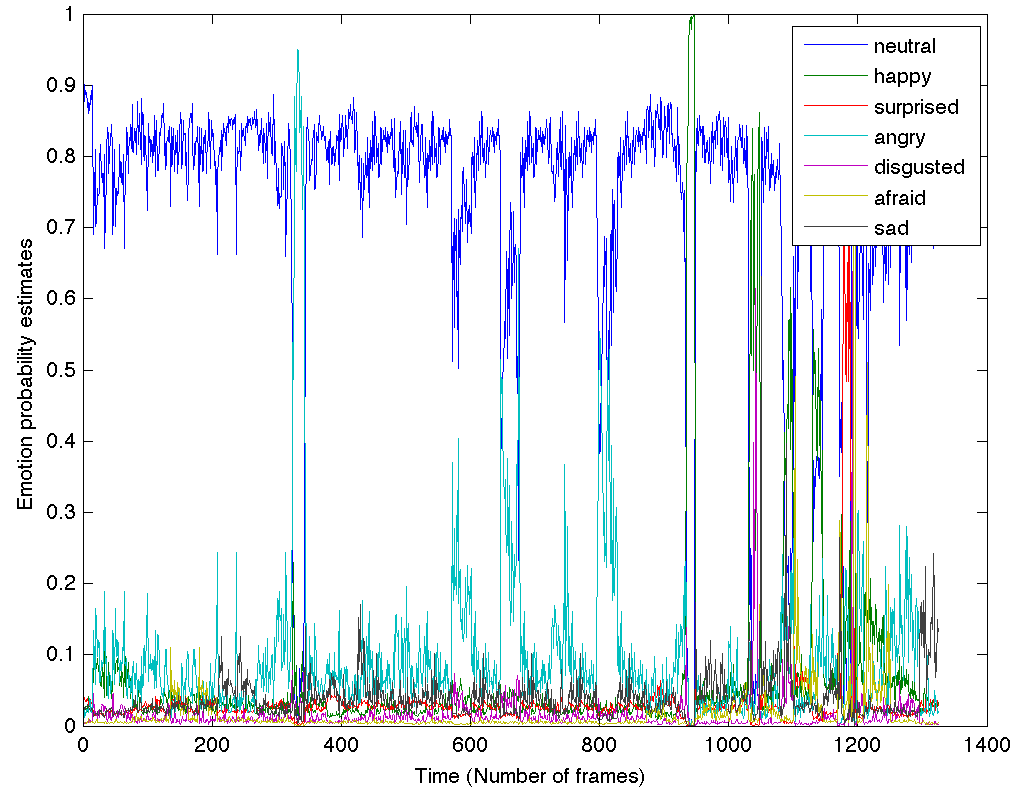
\includegraphics[height=4.7cm,keepaspectratio]{images/paris/sectionStraightEmotions.png}
                \caption{Facial expressions in Straight chunk}
								\label{fig:sectionStraightEmotions}
        \end{subfigure}%
				\quad
        %\\ %add desired spacing between images, e. g. ~, \quad, \qquad etc.
           %(or a blank line to force the subfigure onto a new line)
        \begin{subfigure}[t]{0.32\textwidth}
								\centering
                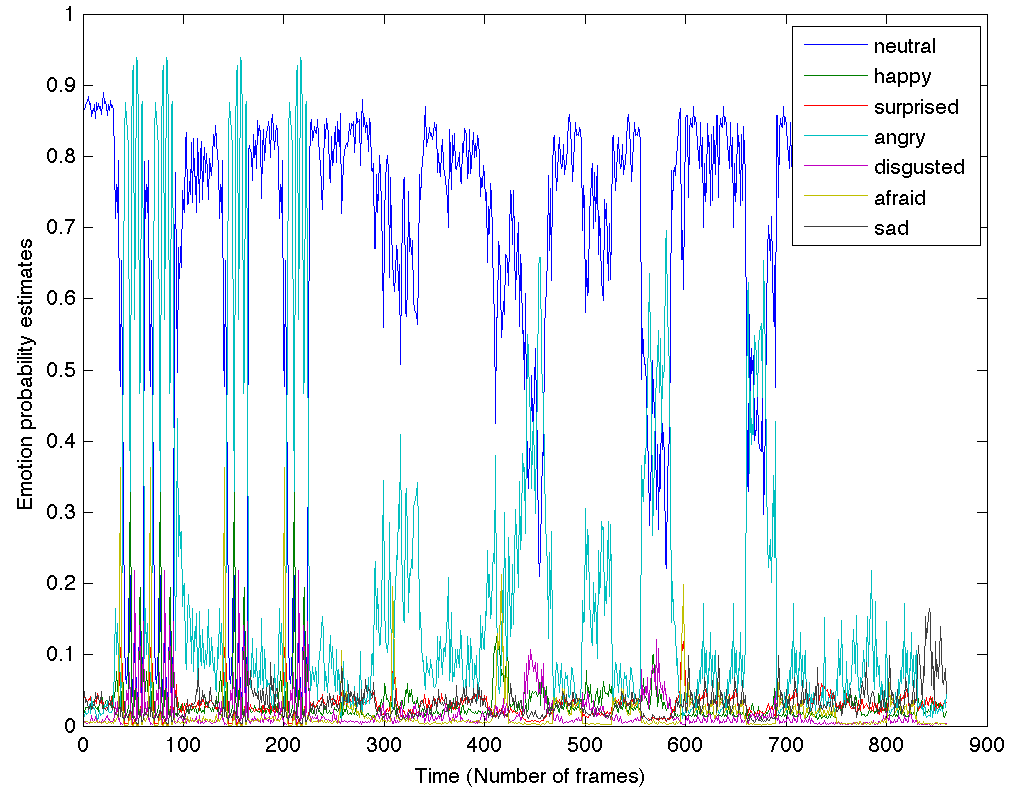
\includegraphics[height=4.7cm,keepaspectratio]{images/paris/sectionHillsEmotions.png}
                \caption{Facial expressions in Hills chunk}
								\label{fig:sectionHillsEmotions}
        \end{subfigure}%
        \\ %add desired spacing between images, e. g. ~, \quad, \qquad etc.
           %(or a blank line to force the subfigure onto a new line)
        \begin{subfigure}[t]{0.32\textwidth}
								\centering
                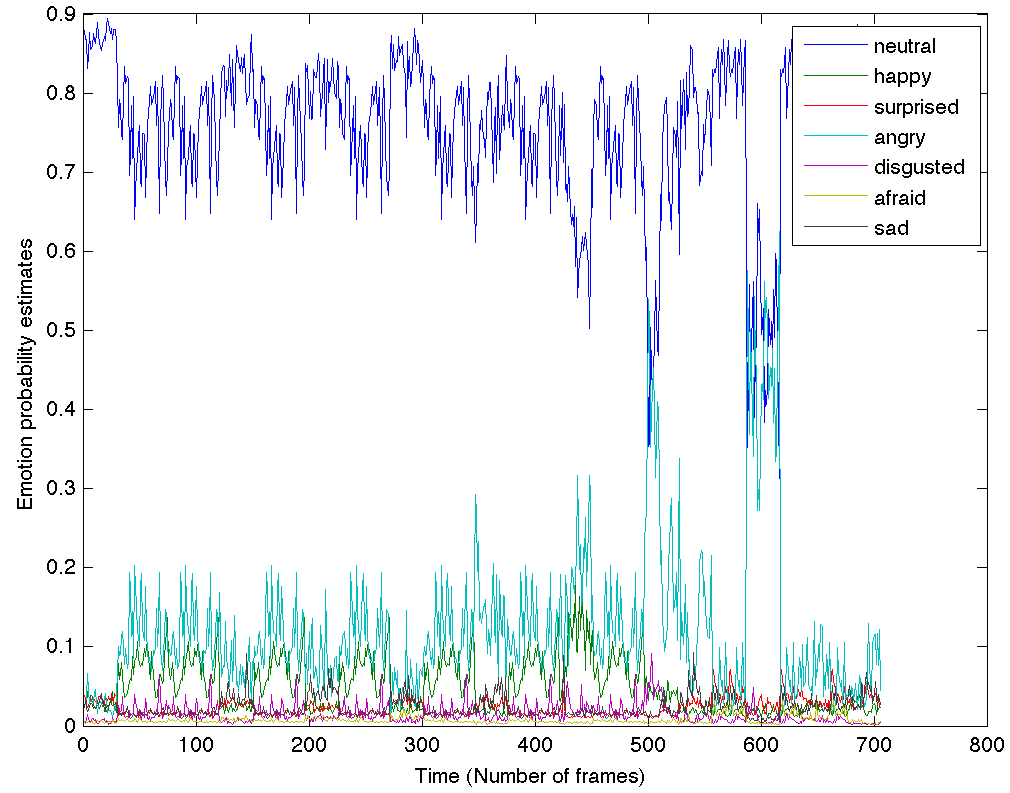
\includegraphics[height=4.7cm,keepaspectratio]{images/paris/sectionTubesEmotions.png}
                \caption{Facial expressions in Tubes chunk}
								\label{fig:sectionTubesEmotions}
        \end{subfigure}%
				\quad
        %\\ %add desired spacing between images, e. g. ~, \quad, \qquad etc.
           %(or a blank line to force the subfigure onto a new line)
        \begin{subfigure}[t]{0.32\textwidth}
								\centering
                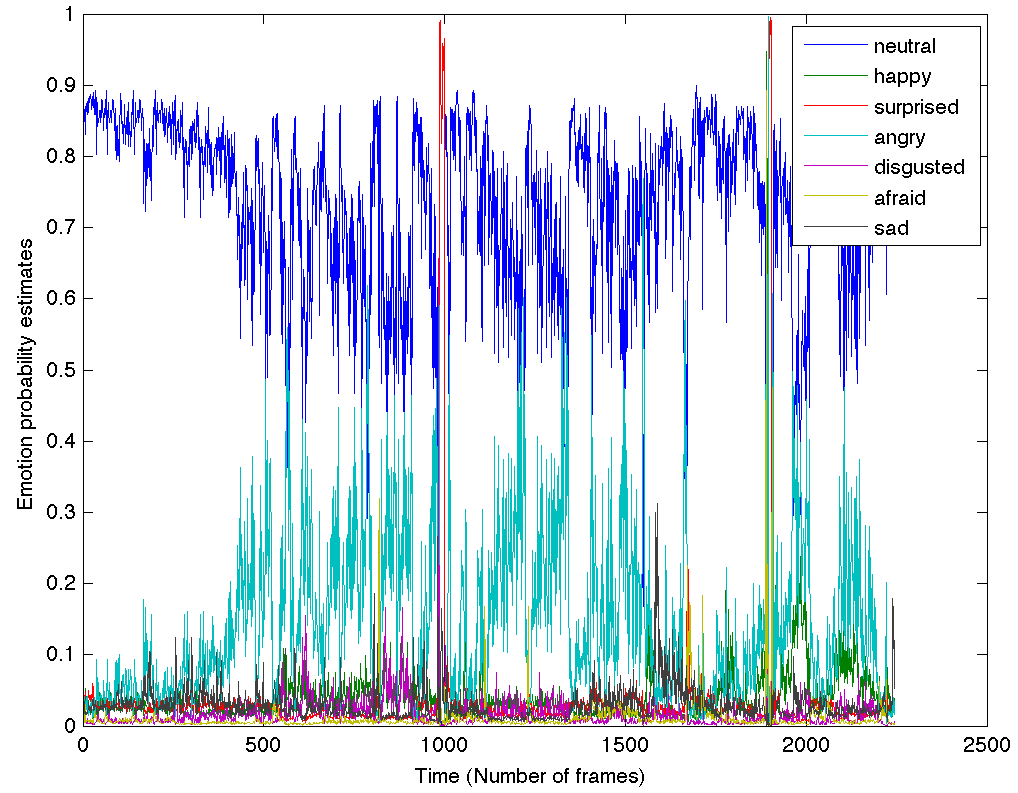
\includegraphics[height=4.7cm,keepaspectratio]{images/paris/sectionJumpsEmotions.png}
                \caption{Facial expressions in Jumps chunk}
								\label{fig:sectionJumpsEmotions}
        \end{subfigure}%
				\quad
        %\\ %add desired spacing between images, e. g. ~, \quad, \qquad etc.
           %(or a blank line to force the subfigure onto a new line)
        \begin{subfigure}[t]{0.32\textwidth}
								\centering
                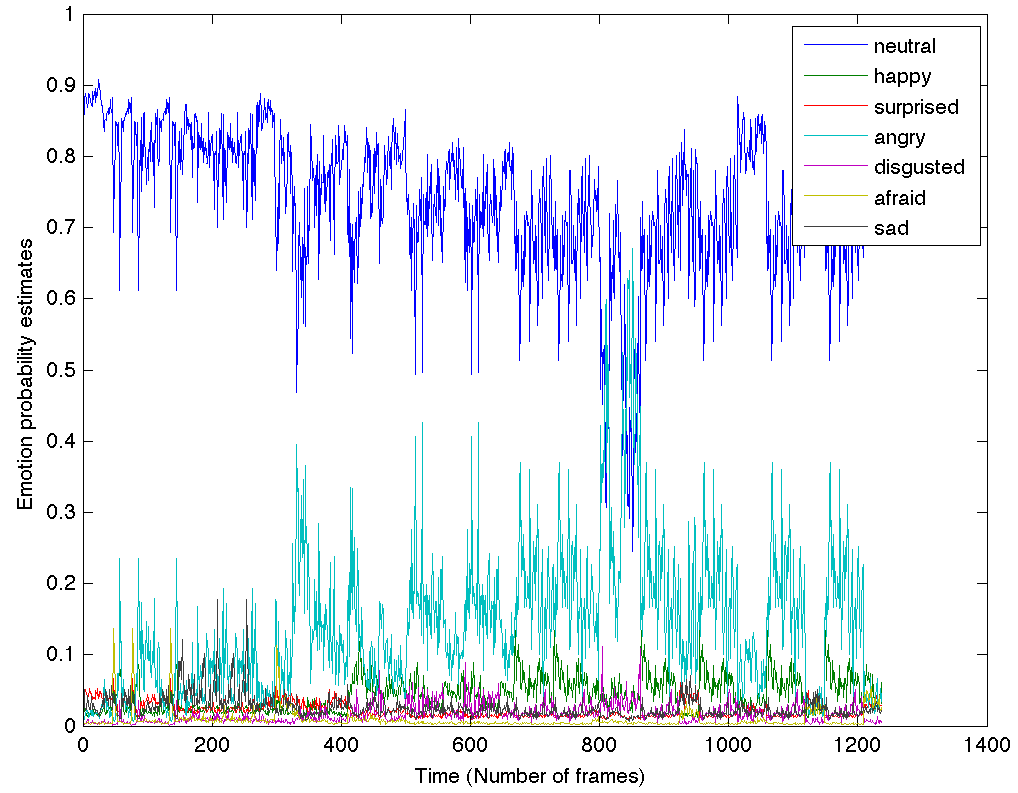
\includegraphics[height=4.7cm,keepaspectratio]{images/paris/sectionCannonsEmotions.png}
                \caption{Facial expressions in Cannons chunk}
								\label{fig:sectionCannonsEmotions}
        \end{subfigure}%
        \caption{Pilot study. Learned challenge parameter values (Figure~\ref{fig:sectionDifficultiesEmotions}) given the measured facial expressions per chunk (Figure~\ref{fig:sectionStraightEmotions} -- \ref{fig:sectionCannonsEmotions}).}
				\label{fig:emotions}
\end{figure*}



\subsection{Online personalisation -- Pairwise tests}\label{exp2}

In this experiment, we investigate how human participants experience the personalised game under actual game playing conditions, in comparison with a realistic (baseline) static game.\footnote{\footnotesize{The static levels are built from chunks of a predetermined challenge level, in random order of occurrence for each new segment, so as to ensure variation and playability. Given this randomisation, the experimental trials are sufficiently short to prevent players from easily noticing possible chunk repetitions.}} To this end, in accordance with procedures employed by Shaker \emph{et al.} \citeyear{shaker2011game}, we query for \emph{pairwise preferences} (i.e., ``is system $A$ preferred over system $B$?''), a methodology with numerous advantages over rating-based questionnaires (e.g., no significant \emph{order of reporting} effects) \cite{yannakakis2011ranking}. We perform pairwise tests of a static system $s$, with a fixed difficulty level, and a personalised system $p$. The experiment follows a \emph{within-subjects design} composed of two randomised conditions (first $s$ then $p$, or inversely), each condition consisting of a series of three sequentially performed pairwise tests, in randomized order. A pairwise test compares the static system vs. the personalised system, both starting at one of the three available challenge levels (easy, normal, or hard).
%. Table~\ref{table:experimentalsetup-3} gives an overview of the resulting experimental conditions, with the initial challenge level of a system indicated between brackets.

%\begin{table}[t]
%\begin{center}
%\caption{Pairwise tests of the static system versus the personalised system. The initial challenge level is indicated between brackets.}
%\scriptsize
%\begin{tabular}{l|ll}
    %\toprule
    %\emph{Initial challenge level} & Condition 1 & Condition 2 \\
    %\midrule
    %\emph{Easy}   & s(easy) vs. p(easy)     & p(easy) vs. s(easy) \\
    %\emph{Normal} & s(normal) vs. p(normal) & p(normal) vs. s(normal) \\
    %\emph{Hard}   & s(hard) vs. p(hard)     & p(hard) vs. s(hard) \\
    %\bottomrule
%\end{tabular}
%\label{table:experimentalsetup-3}
%\end{center}
%\end{table}

The experiment is performed by ten human participants. To minimise user fatigue impacting the experimental results, each of the three game-playing session is ended after a maximum of 4 level segments (i.e., approximately three minutes of play). After completing a pair of two games, we query the participants's preference through a 4-alternative forced choice (4-AFC) questionnaire protocol (e.g., $s$ is preferred to $p$, $p$ is preferred to $s$, both are preferred equally, neither is preferred; both are equally unpreferred). The question presented to the participant is: ``For which game did you find the challenge level more appropriate?''.
%The participant demographics for this experiments were, gender: 27\% female, 73\% male, age: 27 $\pm$ 5 years, hours spent on video games per week: 5 $\pm$ 6 hours, has played Mario before: yes for all participants. We employ the same feedback model, global safe policy, and parameter settings as in Experiment~1.

Table~\ref{table:exp2} lists the pairwise preferences as reported by the human participants. The results reveals that when both gaming systems are set to an initial challenge level of `easy', a significant majority ($p=0.037$) of human participants prefers the personalised system over the static system (70\% over 30\%). Furthermore, we observe that when both gaming systems are set to an initial challenge level of `normal', a significant majority ($p=0.037$) of human participants prefers the personalised system over the static system (also 70\% over 30\%). When both gaming systems are set to an initial challenge level of `hard', a narrow majority 40\% of the human participants prefers the personalised system over the static system (30\%), with the remaining 30\% of the participants preferring neither; both are equally unpreferred.
%in condition 2a, a substantial majority of human participants prefer the personalised system over the static system (62.22\% over 22.22\%), when both systems are initialised with the same policy. In addition, in condition 2b, we observe that when the personalised system is initialised with the learned global safe policy, the preference for this system increases to 68.89\% (while the preference for the static system remains low, at 20.00\%). Finally, in condition 2c, we observe that the personalised system -- initialised with the learned global safe policy -- is preferred over the personalised system with fixed (easy/normal/hard) initialisations, 64.44\% over 28.89\%, respectively.

\begin{table}[t]
\begin{center}
\caption{Pairwise preferences of participants, per initial challenge level. The legenda is a follows, `P' indicates a preference for the personalised system, `S' indicates a preference for the static system, `B' indicates that both are preferred equally, and `N' indicates that neither is preferred; both are equally unpreferred.}
\scriptsize
\begin{tabular}{llll}
    \toprule
    Participant & Easy & Normal & Hard \\
    \midrule
		1 & P & P & S \\
		2 & P & P & N \\
		3 & S & P & P \\
		4 & P & P & N \\
		5 & P & P & P \\
		6 & P & P & S \\
		7 & P & S & S \\
		8 & S & S & N \\
		9 & P & S & P \\
		10 & S & P & P \\
		\midrule
		Totals & \textbf{70\% P} & \textbf{70\% P} & \textbf{40\% P} \\
		       & 30\% S & 30\% S & 30\% S \\
					 & 0\% B  & 0\% B  & 0\% B  \\
					 & 0\% N  & 0\% N  & 30\% N  \\
    \bottomrule
\end{tabular}
\label{table:exp2}
\end{center}
\end{table}

From these results we may conclude that, generally, a majority of human participants prefers the personalised system over the static system. In the case the initial challenge level is `easy' or `normal', it concerns a significant majority. In the case the initial challenge level is `hard', it concerns a narrow majority. A discussion on this latter phenomenon is provided next.
%, and (b) learning an appropriate global safe policy for initialising the game positively affects participant preferences.



%The tables below show the average preferences in difficulty and emotion estimates for 10 players, 3 different setups and 4 segment game sessions.
%
%\begin{table}[t]
%\begin{center}
%\caption{Average emotions estimates for 10 users, over 4 game segments.}
%\scriptsize
%\begin{tabular}{l|{c}*6r}
%Difficulty & Neutral & Happy & Surprised & Angry & Disgusted & Afraid & Sad\\ 
%\hline \\
 %Easy & 0.7261 & 0.0419 & 0.0626 & 0.0967 & 0.0096 & 0.0092 & 0.0539\\
 %Normal & 0.6656 & 0.0619 & 0.0635 & 0.0980 & 0.0189 & 0.0230 & 0.0690\\
 %Hard & 0.7114 & 0.0416 & 0.0689 & 0.1070 & 0.0108 & 0.0095 & 0.0507
%\end{tabular}
%\label{tab:meanEmotions4seg}
%\end{center}
%\end{table}



%\begin{table*}
%\small
%\begin{tabular}{l|{c}*4r}
%Difficulty & Straight & Hills & Tubes & Jumps & Cannons\\
%\hline \\
%Easy & 2.53 & 2.56 & 2.65 & 2.63 & 2.69\\
%Normal & 3.08 & 2.80 & 2.81 & 2.52 & 2.89\\
%Hard & 4.28 & 4.59 & 4.36 & 3.79 & 4.03
%\end{tabular}
%\caption{Average difficulty levels per game chunk for 10 users, over 4 game segments.}
%\label{tab:meanDiffs4seg}
%\end{table*}

\section{Supervised Approach}
The goal of this approach is to further expand the capabilities of the Unsupervised approach, by introducing a trained Random Forest classifier which is meant to predict a user's current challenge level. 

The classifier has been trained by human participants, who provided the system with labeled instances containing a vector of emotion estimates, head pitch, roll \& yaw calculations, the current chunk difficulty, and a likert value attached to each completed chunk. Approximately 1250 instances have been gathered, equally distributed among all game chunks and difficulty levels.

The Supervised system, compared to the unsupervised one, is using head pose information (pitch, roll \& yaw) in order to preserve an accurate estimate of user challenge level even if the user has changed his head pose significantly during gameplay. We believe that head pose information can 'boost' the classification of emotions, given the fact that certain emotions (e.g. anger) could be expressed not only by facial expressions, but also head movement.

The output of the supevised system is a probability distribution over possible likert values [1-5] which leads to one solid estimation using the formula underneath:
\begin{center}
\begin{equation*}
E_{likert} = L[i]*P_{L_i}
\end{equation*}
\end{center}
where, $E_{likert}$ is the estimated likert value, $L[i]$ is the likert class (1,2,3,4,5) and $P_{L_i}$ is the probability estimated by the Random Forest classifier for each likert class $i$ given an unknown instance.

Using this likert estimate, the algorithm fulfils the task of defining the future chunks' difficulties by increasing/decreasing game difficulty according to:
\begin{center}
\begin{equation*}
D_{new} = D_{previous}-(E_{likert}*1.5-4.5)
\end{equation*}
\end{center}
where, $D_{new}$ stands for the future difficulty level and $D_{previous}$ represents the difficulty level of the completed chunk. 
Note that $E_{likert}$ is normalised by $E*1.5-4.5$ in order to scale $D_{new}$ to values $D_{new}\in{-3,3}$.
This scaling factor we found necessary in order to avoid excessively steep changes in game difficulty (e.g. if $D_{previous}=1$ and $E_{likert}=1$, $D_{new} = 5$, which we consider an excessive increase). This way, the maximum achievable increase will be $D_{previous}\pm3$, which is a more realistic approach.

\section{Discussion}\label{sec:discussion}

The pairwise tests revealed that when a gaming system was initialised with a `hard' challenge level, 30\% of the participants preferred neither the static nor the personalised gaming system; both were equally unpreferred. Our data shows that these participants abandoned both the personalised and the static system, presumably because the employed challenge level was consistently too hard. While such user abandonment might be expected in the static system, one would however expect the personalised system to be able to adapt to these circumstances.

Indeed, our personalised system generally \emph{does} decrease the challenge level when it measures the human player being angry. However, in these particular cases, no such measurements were made by the facial expression recognition SDK. We observed that the anger (frustration) of the human participants was not expressed in terms of facial expression, but in terms of hand gesturing, verbal actions, or head movements that prevented facial expressions from being assessed accurately. While this characteristic of the facial expression recognition SDK is outside of our control, we believe that more accurately assessments on player anger can nevertheless be obtained by simultaneously tracking additional features such as gaze and head movement.
%Studying the pairwise testing results, we can detect a decrease in the personalization engine's performance when the initial challenge level is set to 'hard'. However, this occurrence originates from the variety in human behavior and more specifically, anger expression. 
%We could reason that the average user playing at 'hard' challenge level would require the personalization engine to adapt to his skill level by making the game easier. In order for that to happen, GAO has to detect high levels of anger in the user's emotions. However, it is a fact that each user could have his own unique way of expressing anger, including hand gestures, head movement or even verbal actions. On the other hand, \textsc{InSight} only detects anger when a user frowns, which is only one of the aforementioned cases. These facts lead to the conclusion that although the user might be angry, GAO might not be provided with the correct input in order to adapt to that, leading to false classifications, and, as a consequence, false or even no adaptation at all.



\section{Conclusion}\label{sec:conclusion}

In this paper we proposed an approach for personalising the space in which a game is played (i.e., levels) dependent on classifications of the user's facial expression -- to the end of tailoring the affective game experience to the individual user. Our approach is aimed at online game personalisation (i.e., the game experience is personalised \emph{during actual play} of the game). A key insight of this paper is that game personalisation techniques can leverage novel computer vision-based techniques to \emph{unobtrusively} infer player experiences automatically based on \emph{facial expression analysis}. Specifically, to the end of tailoring the affective game experience to the individual user, in this paper we (1) leveraged the established \textsc{InSight} facial expression recognition SDK as a model of the user's affective state \cite{InSight}, and (2) employed this model for guiding the online game personalisation process.
%We contributed an approach that acknowledges that for effective online game personalisation, one needs to rapidly converge to an appropriate policy for the individual user in online gameplay.
%To this end, we (1) utilised the proven \textsc{InSight} facial expression recognition SDK as a model of the user's affective state \cite{InSight}, and (2) employed this model for guiding the online game personalisation process.

The pilot study that tested the online personalisation method indicated that the method operates as expected -- it decreases specific challenge levels in the face of user anger, and increases specific challenge levels in the face of user neutrality or happiness -- and appears stable in the face of classification noise. The pairwise tests across ten human participants revealed that a significant majority of human participants prefers the personalised system over the static system, except in cases when anger (frustration) of the human participants was not expressed in terms of facial expression, but in terms of hand gesturing, verbal actions, or head movements that prevented facial expressions from being assessed accurately. From these results, we may conclude that the developed online personalisation method provides an effective basis for converging to an appropriate affective state for the individual human player.

For future work we will investigate how online game personalisation dependent on a player's facial expressions, can be made more accurate by tracking additional features such as gaze and head movement, and combining it with alternative (multi-objective) feedback models. %Also, the approach could serve as a basis for the multi-objective learning of challenge, frustration, and engagement (cf. the modelling analysis of Shaker \emph{et al.} \shortcite{shaker2011game}). Indeed, the signal richness obtained from facial expression analysis provides a promising start for such an investigation.




%\begin{scriptsize}
%\textbf{Acknowledgements}. The authors would like to thank the following individuals for their valuable input: Frank Nack and Abdo El Ali (setting up user studies), Masrour Zoghi (state-space exploration) and Anne Schuth (random forest classifiers).
%\end{scriptsize}
%%%wish to thank the anonymous referees for their constructive comments that helped to improve the paper considerably.


\clearpage

\begin{spacing}{0.95}
	\begin{footnotesize}
	\bibliographystyle{aaai}
	\bibliography{bibliography_workinprogress}
	\end{footnotesize}
\end{spacing}


\end{document}
